\documentclass[11pt,a4paper]{article}
\usepackage[margin=2.4cm]{geometry}
\usepackage{amsmath,amssymb}
\usepackage{amsthm}
\usepackage{booktabs}
\usepackage{graphicx}
\usepackage{microtype}
\usepackage[hidelinks]{hyperref}
\usepackage{enumitem}

\newtheorem{proposition}{Proposition}
\newtheorem*{definitionstar}{Definition}
\newcommand{\Pesc}{P_{\mathrm{esc}}}
\newcommand{\Pescbar}{\bar{P}_{\mathrm{esc}}}
\newcommand{\clip}{\mathrm{clip}}

\title{\bf Damping from the Escape Probability:\\
a free calibration rule for diffusion-based\\
reachability ranking in uncertain graphs}
\author{Ioannis Konstantellos\\
\small Computer Engineering and Informatics Department\\
\small University of Patras, Greece}
\date{September 2026}

\begin{document}
\maketitle

\begin{abstract}
Damped diffusions---personalised PageRank and its variants---are a standard
cheap heuristic for ranking vertices of a probabilistic graph by expected
reachable mass. Their damping factor $\alpha$ is almost always inherited from
web search ($0.85$) or tuned by grid search against ground truth that is itself
\#P-hard to compute. We show that neither is necessary.

Our contribution is a closed-form calibration. The best-performing $\alpha$ is
predicted by the \emph{mean escape probability} $\Pescbar$, the average
probability that a vertex has at least one incident edge present, which is
already computed when the transition operator is built and is therefore free.
Fitting $\alpha=\clip(0.502+0.558\,\Pescbar,0.4,1)$ on 54 training instances
gives Pearson $r=+0.965$ and out-of-sample mean Spearman $\rho=0.894$,
recovering $98.2\%$ of a per-instance oracle. The rule beats \emph{every} fixed
$\alpha$, including the best one selectable with hindsight on the test set
($0.894$ against $0.677$), because instance densities vary enough that no single
constant serves them. It is a property of the problem rather than of one
operator: refit independently for standard push personalised PageRank it gives
$\clip(0.241+0.859\,\Pescbar)$ with $r=+0.961$ and $98.7\%$ of that family's
oracle. It survives a $14\times$ change of scale without refitting, and on real
citation networks it still beats the best constant $\alpha$, at $91\%$ of oracle.

We also situate the escape probability itself. It is not a new score: it is
exactly the correlation-free ($\eta=1$) zeroth iterate of Karrer, Newman and
Zdeborov\'a's message-passing percolation, and its value is purely one of
engineering. Running that recursion properly is better---on 30 real dense
instances converged message passing reaches $\rho=0.9931$ against $0.9852$ for
the free iterate---and both dominate a 200-sample Monte Carlo ($0.9741$) at a
seventh of its cost. The ranking signal saturates after two iterations. A
reverse-reachable-set estimator from the modern RIS lineage, evaluated in its
singleton-spread form, does not change this picture: at matched budget it
trails plain possible-world sampling for whole-graph ranking, an
information-per-sample effect we quantify and locate. Finally
we report a negative result: routing among heuristics by $\Pescbar$ works on
synthetic graphs and fails on real ones, which we take as evidence that cheap
global density features do not support algorithm selection here. Code and data
are provided.
\end{abstract}

\section{Introduction}

Let $G=(V,E)$ be undirected with $|V|=n$, each edge $(i,j)$ present
independently with probability $p_{ij}\in(0,1]$, and let
$x\in\mathbb{R}^n_{\ge0}$, $\sum_i x_i=1$, be a prior over which vertex is the
target of a routing or search operation. Sampling a world $G'$ and writing
$C(i)$ for the connected component of $i$, we rank vertices by
\begin{equation}
y^*_i \;=\; \mathbb{E}\Big[\textstyle\sum_{v\in C(i)} x_v\Big],
\label{eq:target}
\end{equation}
the expected prior mass reachable from $i$.

\paragraph{What this quantity is.} Equation \eqref{eq:target} is a known object
under two other names, both verified numerically in Section \ref{sec:setup}.

\begin{proposition}[Influence spread]
Under the live-edge equivalence of Kempe, Kleinberg and Tardos \cite{kkt03}, a
vertex is activated by the Independent Cascade model from seed set $S$ exactly
when it is reachable from $S$ in a sampled live-edge graph. For $S=\{i\}$ on an
undirected support reachability is connectivity, so $y^*_i$ is the node-weighted
single-seed expected spread with weights $x$.
\end{proposition}

\begin{proposition}[Percolated component centrality]
With uniform prior and constant edge probability, $n\cdot y^*_i$ is the Edge
Percolated Component score of \cite{hubba08,cytohubba14}.
\end{proposition}

\noindent
Evaluating \eqref{eq:target} exactly subsumes two-terminal network reliability
and is \#P-hard \cite{valiant79,provanball83}, so the field relies on fast
alternatives: structural proxies \cite{degdisc09}, path truncation
\cite{pmia10}, linear-system heuristics \cite{irie12}, sampling estimators with
guarantees \cite{borgs14,tim14,imm15,skim14}, and---the family this paper is
about---damped diffusions.

\paragraph{The gap.} A damped diffusion interpolates between the prior and a
propagated signal,
\[
y \;\leftarrow\; (1-\alpha)\,x \;+\; \alpha\,\mathcal{T}y ,
\]
for a propagation operator $\mathcal{T}$. Personalised PageRank
\cite{pagerank99,haveliwala03} is the canonical instance and variants are
routinely applied to uncertain graphs \cite{kim17,pfeiffer11}. The damping
factor controls how far signal travels before being pulled back toward the
prior, and it is consequential: across our held-out instances, moving $\alpha$
over its range changes mean Spearman $\rho$ by more than $0.2$ for both
operators we study.

Yet $\alpha$ is usually not chosen. It is inherited from web search, fixed by
convention, or---when performance matters---grid searched against ground truth
that is exactly the expensive quantity the heuristic exists to avoid. The same
convention governs current practice: a recent survey of efficient personalised
PageRank computation treats $\alpha$ as a given constant throughout
\cite{yang24}, and PPR-based graph neural networks either fix the teleport
weight or learn propagation weights from labels
\cite{gprgnn21,berberidis19,pirro25}. The damping literature analyses
sensitivity to $\alpha$ \cite{boldi05,bressan10} and ties it to a target
conductance in local partitioning \cite{acl06}. The closest precedents derive
an optimal $\alpha$ in closed form from the parameters of a \emph{planted
model}: Kloumann, Ugander and Kleinberg \cite{kloumann17} obtain
$\alpha^*=(p_{\mathrm{in}}-p_{\mathrm{out}})/(p_{\mathrm{in}}+p_{\mathrm{out}})$
for seed expansion in a stochastic block model, Avrachenkov, Kadavankandy and
Litvak \cite{avrachenkov18} an optimum from the same model's density ratio, and
Li, Chien and Milenkovic \cite{li19gpr} optimal generalized-PageRank weights
under related generative assumptions. While prior work has theoretically attempted
to estimate planted model parameters from the graph (e.g., using the Allman et
al.\ estimator \cite{allman11}), such methods require known block sizes and are
notoriously brittle on non-SBM graphs. In contrast, our $\Pescbar$ calibration
operates directly on the topology of any real network without requiring block
assumptions, and is computed for free when the operator is built.

\paragraph{Contributions.}
\begin{enumerate}[leftmargin=1.5em,itemsep=2pt]
\item \textbf{A free damping calibration} (Sections
\ref{sec:rule}--\ref{sec:results}), the main result: $\alpha$ predicted from
$\Pescbar$ at $r=+0.965$, recovering over $98\%$ of a per-instance oracle,
beating every constant including the hindsight-best, transferring across
operator families and across a $14\times$ change of scale, and robust to
rounding its coefficients.
\item \textbf{An honest placement of the escape probability} (Section
\ref{sec:mp}). $\Pesc$ is the $\eta=1$ zeroth iterate of message-passing
percolation \cite{knz14}; we say so, implement the full recursion as the proper
deterministic competitor, and show the ranking signal saturates after two
iterations while both dominate small-budget sampling. We also benchmark a
reverse-reachable-set estimator from the modern RIS lineage
\cite{borgs14,imm15,guo20,guo22} in its singleton-spread form (Section
\ref{sec:rr}), and locate why it trails the possible-world estimator for
whole-graph ranking at matched budget.
\item \textbf{A negative result on algorithm selection} (Section
\ref{sec:router}). Routing among heuristics by $\Pescbar$ beats the best single
method on synthetic graphs and fails outright on real citation networks. We
report the failure rather than the synthetic-only success.
\end{enumerate}

\section{The escape probability, and what it is}
\label{sec:pesc}

\begin{definitionstar}
$\Pesc(i)=1-\prod_{j\in N(i)}(1-p_{ij})$ is the probability that vertex $i$ has
at least one incident edge present---that it is not isolated in a sampled
world. We write $\Pescbar=\frac1n\sum_i\Pesc(i)$.
\end{definitionstar}

\noindent
The expression is not new and we make no claim on it. It is the one-hop case of
the activation recursion in MIA/PMIA \cite{pmia10}, the complement of the node
isolation probability studied in wireless connectivity \cite{takabe18}, and the
per-node summand of the giant-component size in percolation theory. Most
precisely:

\paragraph{$\Pesc$ is the correlation-free limit of message-passing percolation.}
Karrer, Newman and Zdeborov\'a \cite{knz14} compute, deterministically, the
probability that each vertex belongs to the giant cluster. In membership
variables their recursion reads
\begin{equation}
\nu_{i\to j} \;=\; 1-\!\!\prod_{k\in N(i)\setminus j}\!\!\big(1-p_{ik}\,\nu_{k\to i}\big),
\qquad
\mu_i \;=\; 1-\!\prod_{k\in N(i)}\!\big(1-p_{ik}\,\nu_{k\to i}\big).
\label{eq:mp}
\end{equation}
Initialising $\nu\equiv1$ and evaluating $\mu$ once, with no message updates,
gives $\mu_i=1-\prod_k(1-p_{ik})=\Pesc(i)$ exactly. The escape probability is
therefore the zeroth iterate of \eqref{eq:mp} under the assumption that every
present edge leads to the giant cluster. Equivalently, for constant $p$ and
degree $k$ it is the $u\to0$ case of the $1-u^k$ membership probability in the
generating-function formalism of Newman, Strogatz and Watts \cite{nsw01} and
Callaway et al.\ \cite{callaway00}. We verify the identity numerically
(Section \ref{sec:mp}).

The consequence for this paper is a demotion and a clarification. $\Pesc$ is
not a mechanism we discovered; it is a known quantity in its most degenerate
form. Its interest here is purely one of engineering: it costs one pass over
the edge list, which building any transition operator already performs, so it is
free in a sense that no iterated quantity is. That is why we use it as the
feature for the calibration rule, and it is the only property of it we rely on.
$\Pescbar$ is also a smooth, bounded measure of \emph{effective} density---it
approaches $0$ when vertices are typically isolated and $1$ when they are
typically connected, and unlike average degree it accounts for edge reliability.

\section{The calibration rule}
\label{sec:rule}

Let $W$ be row-stochastic on the potential adjacency with
$W_{ij}\propto-\ln(1-p_{ij})$ (Section \ref{sec:results} shows the weighting is
immaterial). We study two damped diffusions: standard push personalised
PageRank \cite{pagerank99,haveliwala03},
\begin{equation}
y \;\leftarrow\; \mathrm{normalise}\big[(1-\alpha)x + \alpha\,W^{\!\top}y\big],
\label{eq:push}
\end{equation}
and an escape-scaled pull form in which each vertex is attenuated by its own
escape probability, making the operator sub-stochastic,
\begin{equation}
y \;\leftarrow\; \mathrm{normalise}\big[(1-\alpha)x + \alpha\,(\Pesc\odot(Wy))\big],
\label{eq:pull}
\end{equation}
a mild instance of the partially absorbing random walk \cite{wu12} with
absorption set by edge reliability. Both need an $\alpha$, and the value that
maximises rank correlation varies systematically with how connected the sampled
worlds tend to be. Sparse instances need small $\alpha$: components are small
and $y^*$ is close to $x$. Dense instances need large $\alpha$: the prior is
nearly irrelevant and the propagated structure carries the signal. $\Pescbar$
measures exactly this axis.

We calibrate on 54 instances at $n=64$ (Erdős--Rényi, Barabási--Albert and grid
topologies; six probability ranges; three seeds). For each we grid search the
$\alpha$ maximising Spearman $\rho$ against Monte-Carlo ground truth, then
regress it on $\Pescbar$. Least squares gives
\begin{equation}
\boxed{\;\alpha \;=\; \clip\!\left(0.502 + 0.558\,\Pescbar,\; 0.4,\; 1.0\right)\;}
\label{eq:rule}
\end{equation}
with Pearson $r=+0.965$ ($p=5.9\times10^{-32}$), Spearman $+0.959$, and residual
RMSE $0.043$ (Figure \ref{fig:alpha}(a)). The lower clip never binds; it is
retained for degenerate inputs. Since $\Pescbar$ is available at initialisation,
\eqref{eq:rule} adds no measurable cost.

\section{Experimental setup}
\label{sec:setup}

\paragraph{Ground truth.} Monte Carlo over sampled worlds, extracting connected
components with SciPy's sparse graph routines; 3{,}000 samples per held-out
instance, 2{,}500 during calibration. Significance is paired Wilcoxon
signed-rank; confidence intervals are bootstrap percentile intervals over
$20{,}000$ resamples. Timings are single-core wall clock.

\paragraph{Identity checks.} On an $n=60$ instance the maximum discrepancy
between $y^*$ and an independently simulated single-seed Independent Cascade
with node weights is $0.0058$, against Monte-Carlo noise of $1/\sqrt{4000}=
0.0158$. With uniform prior and constant $p$, $n\cdot y^*$ reproduces the EPC
score at Spearman $1.000000$. Propositions 1 and 2 hold as stated.

\paragraph{Synthetic instances.} A held-out set of 100 instances at $n=100$
(four topologies including Watts--Strogatz, absent from calibration; five
probability ranges; five seeds). A stratified panel of 400 instances at $n=900$
built for coverage: $(0,1]$ divided into eight equal-width strata of $\Pescbar$
with 50 instances each, and within a stratum every other factor randomised
(topology, average degree over $\{4,\dots,12\}$, probability range, prior type,
seed). Design matters here and we can show it rather than assert it: operators
\eqref{eq:push} and \eqref{eq:pull} are indistinguishable under the $n=100$ grid
design ($p=0.60$) and separated at $p=1.5\times10^{-21}$ under the stratified
one; running the identical stratified design at $n=100$ reproduces the
separation ($p=1.7\times10^{-10}$), so the cause is balanced coverage of the
density axis, not scale.

\paragraph{Real networks.} Three genres, seven base graphs. Citation: Cora
($n=2708$), CiteSeer ($3279$), PubMed ($19717$) from the Planetoid release plus
their $k$-cores. Co-purchase: Amazon Computers ($13752$) and Photo ($7650$).
Co-authorship: Microsoft Academic CS ($18333$) and Physics ($34493$). Degree
heterogeneity is far beyond the synthetic families (coefficient of variation
$0.77$--$1.97$) and clustering runs $0.14$--$0.40$ against $\approx0$ for
Erdős--Rényi. Edge probabilities are assigned---no dataset carries observed
$p_{ij}$---by uniform ranges and by the weighted-cascade rule
$p_{ij}=1/\max(\deg_i,\deg_j)$, which is out of distribution for our rule.
Subgraphs are snowball samples, which preserve local density where a random node
sample would artificially sparsify.

\begin{figure}[htbp]
\centering
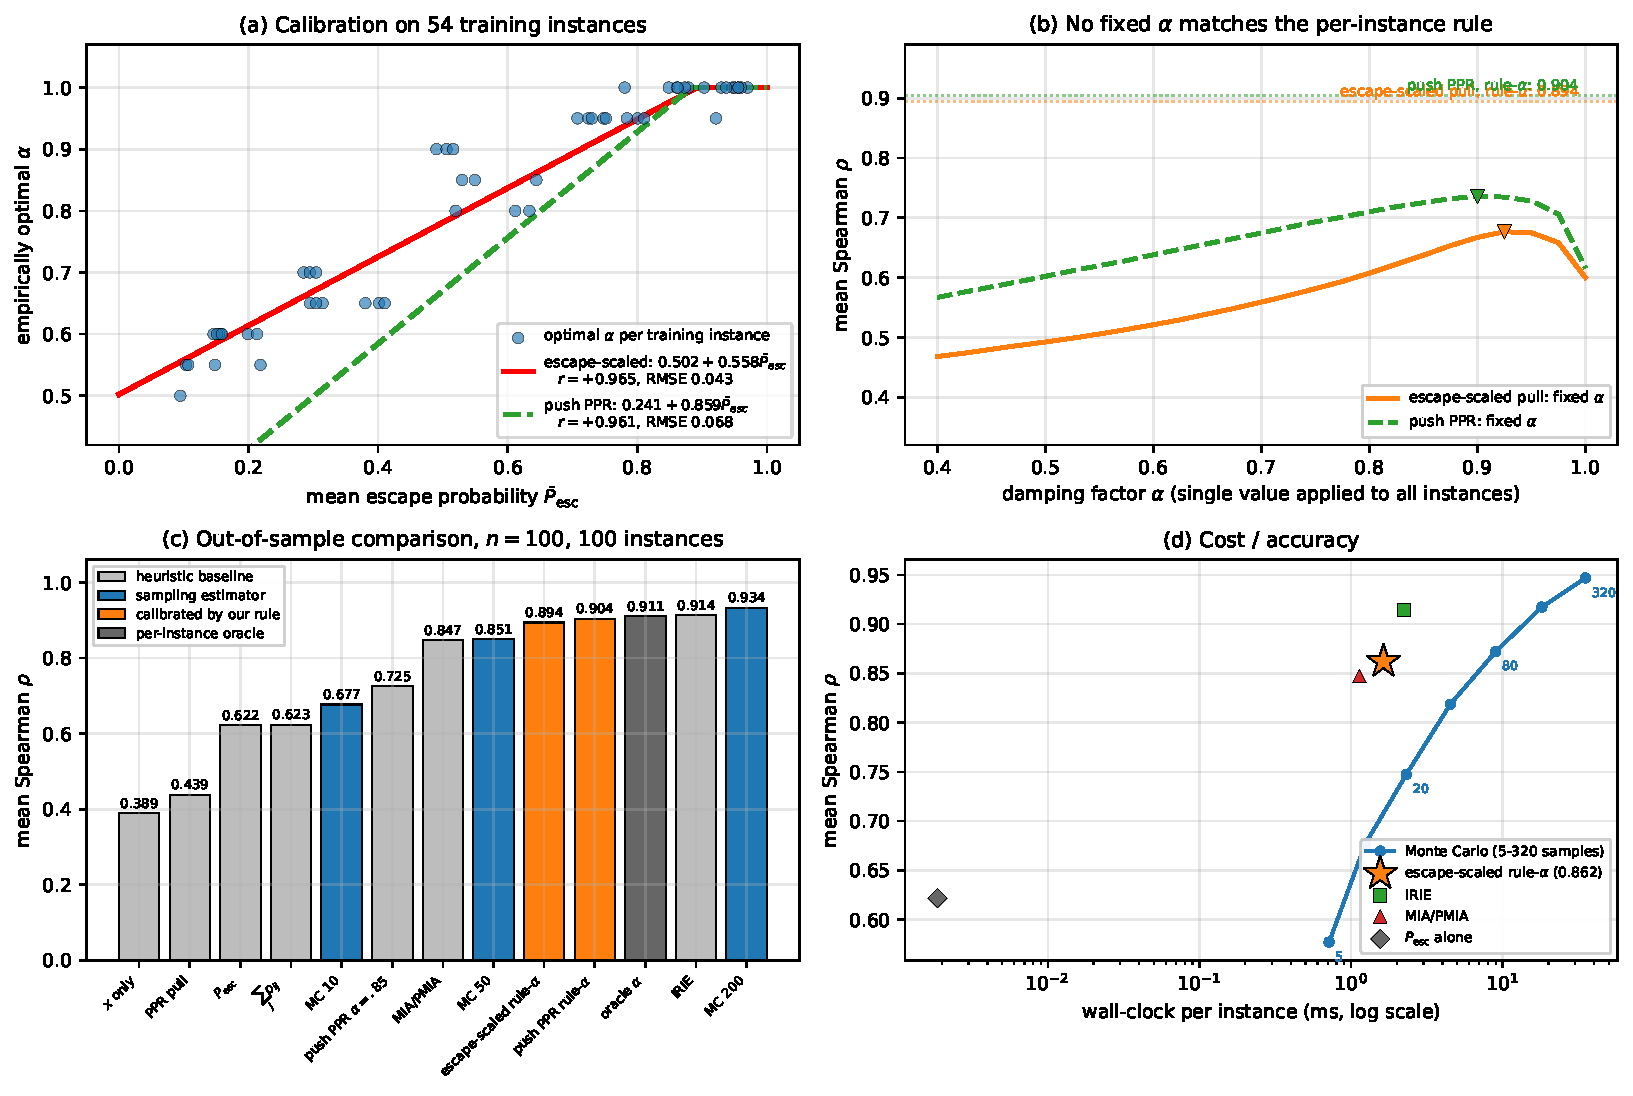
\includegraphics[width=\textwidth]{fig1.pdf}
\caption{\textbf{(a)} The calibration, fitted independently for two operator
families. \textbf{(b)} Out-of-sample mean $\rho$ as a function of a single fixed
$\alpha$ applied to all instances; triangles mark the best attainable constant,
dotted lines the per-instance rule. \textbf{(c)} Comparison against
influence-ranking baselines at $n=100$. \textbf{(d)} Accuracy against wall
clock.}
\label{fig:alpha}
\end{figure}

\section{Results: the calibration}
\label{sec:results}

\subsection{No fixed damping factor is adequate}

Figure \ref{fig:alpha}(b) sweeps a single $\alpha$ applied uniformly to all 100
held-out instances. The best attainable value is $\rho=0.677$ at $\alpha=0.925$
for the escape-scaled operator and $0.736$ at $\alpha=0.900$ for push PPR---both
chosen with hindsight on the test set, and therefore an upper bound on any
constant-$\alpha$ policy. The per-instance rule attains $0.894$ and $0.904$:
margins of $+0.217$ and $+0.168$ over the best possible constant. The
conventional $\alpha=0.85$ gives $0.637$ and $0.725$.

The interpretation is direct. Our instance pool spans effective densities from
near-isolation to near-complete connectivity, the optimal $\alpha$ moves across
most of its range in response, and no single value serves both ends. What makes
this actionable is that $\Pescbar$ locates an instance on that axis at no cost.

\subsection{The rule describes the problem, not one operator}

\begin{table}[h]
\centering\small
\caption{The calibration refit independently per operator family on the same 54
instances. ``\% oracle'' is rule performance as a fraction of a per-instance
oracle over the same $\alpha$ grid.}
\label{tab:transfer}
\begin{tabular}{lccccc}
\toprule
operator family & fitted rule & $r$ & $\alpha{=}0.85$ & rule-$\alpha$ & \% oracle \\
\midrule
escape-scaled pull \eqref{eq:pull} & $\clip(0.502+0.558\,\Pescbar)$ & $+0.965$ & 0.637 & \textbf{0.894} & 98.2\% \\
push PPR \eqref{eq:push}           & $\clip(0.241+0.859\,\Pescbar)$ & $+0.961$ & 0.725 & \textbf{0.904} & 98.7\% \\
IRIE, row-normalised \cite{irie12} & $\clip(0.292+0.593\,\Pescbar)$ & $+0.767$ & 0.404 & 0.439 & 94.8\% \\
\bottomrule
\end{tabular}
\end{table}

For the two teleportation-style diffusions the correlation exceeds $+0.96$ and
the rule recovers over $98\%$ of oracle, with slopes that differ---as they
should, since the operators propagate at different rates---but the same
near-linear dependence on $\Pescbar$. On Watts--Strogatz instances, a topology
family never used in calibration, the rule attains $\rho=0.998$, $0.994$ and
$0.977$ in the three sparsest regimes. The third row marks the limit of its
reach: IRIE's row-normalised variant has a different fixed-point structure and
the relationship is materially weaker. We report it rather than omit it.

\subsection{Scale, robustness, and where it stops working}

Applied unchanged to the 400-instance panel at $n=900$, the correlation weakens
($r=+0.603$ and $+0.719$) while the usefulness does not: the rule still recovers
$95.5\%$ and $94.7\%$ of oracle and beats the best constant $\alpha$ by $+0.067$
and $+0.083$. The reason is measurable rather than rhetorical---the fraction of
the $\alpha$ grid within $0.005$ of an instance's own optimum grows from $0.147$
at $n=64$ to $0.290$ at $n=900$, so the optimum is $1.97\times$ flatter and its
location correspondingly noisier while the penalty for missing it shrinks.
Refitting on the $n=900$ data barely helps (RMSE $0.150\to0.147$).

Sensitivity to the coefficients is asymmetric. Rounding to
$\alpha=\clip(0.5+0.6\,\Pescbar)$ costs $0.009$; raising the intercept by $0.10$
costs $0.031$ and the slope by $0.20$ costs $0.038$; lowering them costs $0.199$
and $0.283$. The $\rho$-versus-$\alpha$ curve is steep below its optimum and
flat above it, so a practitioner uncertain of the coefficients should err
upward, and the round numbers are a serviceable substitute for the fitted ones.

On the 35 real citation instances, applied without refitting, the rule gives
$\rho=0.788$ against $0.765$ for the best constant $\alpha$ selectable with
hindsight, and $0.669$ against $0.622$ for push PPR---so it still beats every
fixed $\alpha$, at $91\%$ and $89\%$ of a per-instance oracle. But the
correlation that motivated it does not survive: optimal $\alpha$ correlates with
$\Pescbar$ at $r=+0.225$ and $+0.623$ there. The rule continues to select good
damping factors on real graphs largely because it selects \emph{high} ones, and
high ones are right on these networks. The synthetic panels show the rule is
not reducible to ``always choose a high $\alpha$''---there the best fixed
$\alpha$ is itself high ($0.925$) and still reaches only $0.677$ against the
rule's $0.894$---but on these real networks the upper clip does much of the
work, and we say so. We report the calibration as empirically useful and
mechanistically unconfirmed outside the synthetic regime.

\paragraph{Ablation: edge weighting.} Logarithmic, linear and uniform weights
give $0.8940$, $0.8931$ and $0.8881$ under \eqref{eq:rule}. The weighting scheme
is not load-bearing.

\paragraph{Per-node damping does not follow from $\Pesc$.} Optimising the
$\alpha$ vector directly by coordinate ascent, and scoring it against an
\emph{independent} ground-truth estimate to exclude overfitting, yields $+0.062$
over the scalar oracle, only $11\%$ of the apparent gain being overfit. But it
does not come from $\Pesc$: setting $\alpha_i=\clip(c_0+c_1S_i)$ with $S$ the
neighbourhood-smoothed escape probability at decay $\beta$ gives $0.867$ at
$\beta=0$, $0.885$ at $\beta=0.5$ and $0.894$ at $\beta=0.9$---monotonically
worse the more local it becomes. The diagnostic is the grid family, where all
$\Pesc(i)$ are nearly equal so a local rule has no variation to exploit, yet the
per-node oracle still gains $+0.341$. The exploitable per-vertex signal is
structural, not escape-based.

\section{The escape probability against message passing}
\label{sec:mp}

Since $\Pesc$ is the zeroth iterate of \eqref{eq:mp}, the honest deterministic
competitor is that recursion run properly, not a sampling estimator. We
implement it and report the comparison. Products are evaluated in log space and
the excluded-neighbour term removed by subtraction, which is stable as
$p\nu\to1$.

\begin{figure}[htbp]
\centering
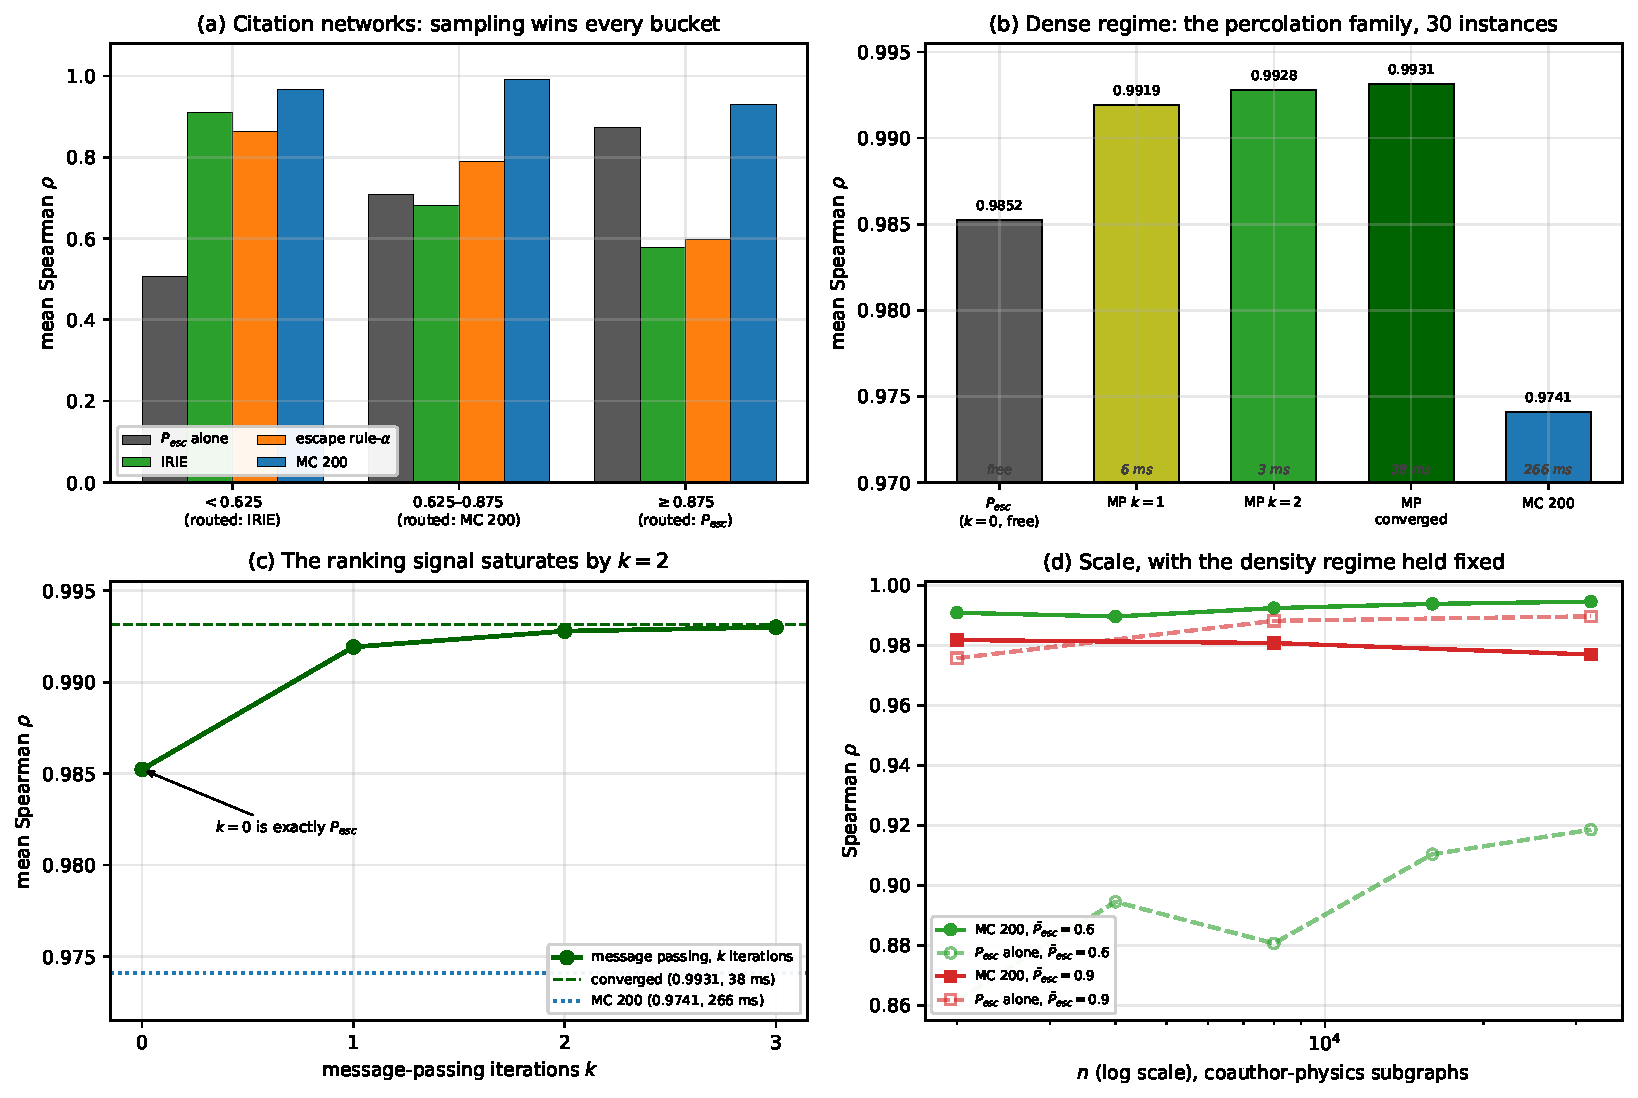
\includegraphics[width=\textwidth]{fig4.pdf}
\caption{\textbf{(a)} On citation networks, sampling wins every bucket of the
routing rule (Section \ref{sec:router}). \textbf{(b)} The deterministic
percolation family against sampling on 30 real dense instances; costs beneath
each bar. \textbf{(c)} The ranking signal as a function of message-passing
iterations; $k=0$ is exactly $\Pesc$. \textbf{(d)} Size sweep with the density
regime held fixed by tuning the edge probability.}
\label{fig:real}
\end{figure}

On 30 instances drawn from co-purchase and co-authorship networks at
$\Pescbar=0.90$, with $n$ from $10^3$ to $1.6\times10^4$:

\begin{center}\small
\begin{tabular}{lrrrr}
\toprule
method & mean $\rho$ & mean ms & vs $\Pesc$ & $p$ \\
\midrule
$\Pesc$, i.e.\ $k=0$      & 0.9852 & $\approx0$ & --- & --- \\
message passing, $k=1$    & 0.9919 & 6.0 & $+0.0067$ & $1.9\times10^{-9}$ \\
message passing, $k=2$    & 0.9928 & 3.2 & $+0.0076$ & $1.9\times10^{-9}$ \\
message passing, converged& \textbf{0.9931} & 38.0 & $+0.0079$ & $1.9\times10^{-9}$ \\
Monte Carlo, 200 samples  & 0.9741 & 266.2 & $-0.0111$ & $4.2\times10^{-4}$ \\
\bottomrule
\end{tabular}
\end{center}

\noindent
Three things follow, and only the third is ours.

First, \textbf{message passing beats its own $\eta=1$ limit}, by $+0.0079$ with
$p=1.9\times10^{-9}$. Any claim that $\Pesc$ is the right deterministic score
for this regime is therefore wrong, and we do not make it. If three
milliseconds are available, iterate.

Second, \textbf{the deterministic family beats sampling}, decisively: converged
message passing outranks a 200-sample Monte Carlo by $+0.0191$, winning $29/30$
($p=9.3\times10^{-9}$), at a seventh of the cost. This is the expected
consequence of a point Newman makes directly \cite{newman23}---simulation yields
an approximate answer subject to sampling error where message passing yields the
value---and we record it as confirmation rather than as a finding.

Third, and this we do offer: \textbf{the ranking signal saturates almost
immediately}. Two iterations reach within $0.0003$ of convergence at a twelfth
of the cost, and the free zeroth iterate is already within $0.008$. For
\emph{ranking} in the dense regime the correlations that message passing corrects
are largely rank-preserving. A practitioner needing a score during operator
initialisation can use $\Pesc$ and lose under one percent of a Spearman
correlation; one who can afford two sparse sweeps should take them.

We did not test message passing outside the dense regime, where its fixed point
is less well behaved on finite graphs, nor against the non-backtracking and
collective-influence rankings that occupy the neighbouring literature
\cite{radicchi16,morone15}. We also note that recent work questions what these
message-passing solutions identify on graphs with cycles \cite{hiraoka26}.

\section{A modern sampling baseline: reverse-reachable sets}
\label{sec:rr}

The sampling side of the comparison so far is plain possible-world Monte
Carlo. The modern sampling machinery for influence, however, is the
reverse-reachable-set (RR-set) framework \cite{borgs14,tim14,imm15}, whose
current generation---SUBSIM and its successors---improves RR-set construction
by up to an order of magnitude and remains the state of the art with
guarantees \cite{guo20,guo22,li23survey}. A comparative study of this problem
should include it, so we do.

\paragraph{The estimator.} Sample a root $r\sim x$; sample a possible world
lazily; the reverse-reachable set of $r$ on an undirected support is
$\mathrm{RR}(r)=C(r)$. Then
$\mathbb{E}[\,\mathbf{1}\{i\in \mathrm{RR}\}\,]=\sum_r x_r\,P(i\sim r)=y^*_i$
exactly, so the fraction of $\theta$ sets containing $i$ is an unbiased
estimate of the objective---the singleton-spread special case of RR-set
sampling, with the root drawn from the prior as in weighted variants
\cite{kbtim15}. Our implementation generates sets lazily and
level-synchronously: only edges incident to the growing set are examined, each
undirected edge at most once, with the Bernoulli draws vectorised over the
frontier---the subset-sampling idea behind modern RR-set generators
\cite{guo20,guo22} in array form. Correctness was verified against ground
truth ($\theta=6\times10^4$ reproduces $y^*$ to within Monte-Carlo noise).

\begin{table}[h]
\centering\small
\caption{The RR-set estimator against possible-world Monte Carlo on all three
panels. Same instances and ground truth as the preceding sections; costs are
mean wall clock. The rule-$\alpha$ row is the calibrated diffusion of Section
\ref{sec:results}, for context.}
\label{tab:rr}
\begin{tabular}{l rr rr rr}
\toprule
& \multicolumn{2}{c}{synthetic, $n{=}100$ (100)} & \multicolumn{2}{c}{citation (35)} & \multicolumn{2}{c}{dense real (30)} \\
method & $\rho$ & ms & $\rho$ & ms & $\rho$ & ms \\
\midrule
escape-scaled rule-$\alpha$ & 0.894 & 2.2 & 0.788 & 13 & --- & --- \\
Monte Carlo, 200 worlds     & 0.934 & 28  & 0.964 & 87 & 0.974 & 265 \\
RR sets, $\theta=200$       & 0.801 & 31  & 0.641 & 99 & 0.972 & 556 \\
RR sets, $\theta=800$       & 0.924 & 123 & 0.738 & 386 & 0.989 & 2251 \\
RR sets, $\theta=3200$      & 0.970 & 493 & --- & --- & --- & --- \\
\bottomrule
\end{tabular}
\end{table}

\paragraph{At matched budget, the possible-world estimator wins for
whole-graph ranking.} On the synthetic hold-out, RR at $\theta=200$ trails MC
at 200 worlds by $-0.133$ at the same wall clock ($p=3.9\times10^{-16}$,
losing 96/100); roughly $16\times$ the sets are needed to draw level. On the
citation networks the gap is $-0.323$ ($p=2.9\times10^{-10}$), driven by a
collapse in the sparse bucket (RR-200 mean $\rho=0.409$ against MC-200's
$0.968$ over 20 instances). The cause is information per unit of work, and it
is structural rather than an implementation artefact. One sampled world yields
component labels for \emph{every} vertex simultaneously, so all $n$ estimates
share it; one RR set yields a single containment bit per vertex, and in sparse
regimes---where components are small---most vertices appear in no set at all
after hundreds of draws and are left tied at zero. RR sets are the right
primitive for what they were designed for, top-$k$ seed selection with
$(\varepsilon,\delta)$ guarantees on $\sigma(S)$; for ranking \emph{all}
vertices they are dominated at matched budget.

\paragraph{The dense regime inverts the picture, and the deterministic family
wins it anyway.} At $\Pescbar=0.90$ each RR set is nearly the whole giant
component, so per-set information is high: RR-200 ties MC-200 ($0.972$ vs
$0.974$) and RR-800 beats it ($+0.015$, winning 30/30, $p=1.9\times10^{-9}$)
at $8.5\times$ its cost. But RR-800 does not significantly beat the free
zeroth iterate $\Pesc$ ($+0.004$, $p=0.34$) at four orders of magnitude more
cost, and converged message passing (Section \ref{sec:mp}) outranks it
outright at $1/59$ of its wall clock ($0.9931$ at $38$\,ms against $0.9889$ at
$2251$\,ms). In the one regime where RR sets are informative per unit cost,
deterministic percolation is better still.

\paragraph{Positioning among modern estimators.} Learning-based influence
estimators are the other modern family \cite{li23survey}: DeepIS propagates
Independent-Cascade probabilities in a PPNP-like architecture \cite{deepis21},
MONSTOR and GLIE learn inductive GNN surrogates of the spread
\cite{monstor20,glie23,ling23,chowdhury24}, and deep reinforcement learning
attacks seed selection directly \cite{piano23,touplegdd24}. We cite their own
reported costs rather than estimate any: GLIE trains on a 12\,GB GPU with
grid-searched hyperparameters and reports reliable generalisation to graphs up
to roughly ten times its training size \cite{glie23}; DeepIM reports training
times of order $10^3$ seconds on a 50{,}000-node graph and out-of-memory
failures for the RL-based PIANO and ToupleGDD on its largest datasets
\cite{ling23}; ToupleGDD trains on a 16\,GB V100 \cite{touplegdd24}. None of
this is prohibitive, but all of it is infrastructure---labelled training data
(typically generated by Monte-Carlo simulation), a GPU, and a tuning
protocol---and these methods target seed-\emph{set} maximisation rather than
whole-graph single-seed ranking, so we cite them for context rather than run
them. One structural connection is worth recording: the one-hop activation
expression $1-\prod(1-p)$ at the base of GLIE's first message-passing layer
\cite{glie23} is exactly the escape probability of Section \ref{sec:pesc}.
The calibration of Section \ref{sec:rule} is therefore not a competitor to
trained estimators but the zero-parameter end of the same design space: a
closed-form, CPU-only, $O(|E|)$ default for the diffusion family they are
benchmarked against, in a query-processing practice that, as recent work
notes, still relies primarily on Monte-Carlo sampling and heuristics
\cite{wang24}, with RR-set construction itself remaining the bottleneck in
adaptive settings \cite{guo23}.

\section{A negative result: algorithm selection}
\label{sec:router}

No method above wins everywhere on synthetic graphs, and the leader changes
systematically with density: IRIE below $\Pescbar\approx0.63$, Monte Carlo
between $0.63$ and $0.88$, and $\Pesc$ used directly above that. Since
$\Pescbar$ is free and available before any algorithm runs, an obvious idea is
to route on it. We tried, and report the outcome because it is negative.

On the 400-instance synthetic panel a three-bucket rule---IRIE below $0.625$,
Monte Carlo to $0.875$, $\Pesc$ above---reaches $\rho=0.9477$ under 5-fold
cross-validation against $0.9166$ for the best single method ($p=0.009$),
capturing $59\%$ of the gain a per-instance oracle selector would obtain. Three
buckets suffice; eight do no better and sixteen begin to overfit. Thresholds
fitted at $n=900$ transfer to $n=100$ unchanged ($0.9524$ against $0.9527$ fitted
natively).

\textbf{On real citation networks it fails.} Over 35 instances the router scores
$0.9176$ against $0.9637$ for simply running a 200-sample Monte Carlo
everywhere. Figure \ref{fig:real}(a) shows why: sampling wins \emph{every}
bucket---$0.968$ against IRIE's $0.910$ in the sparse bucket, $0.992$ in the
middle, $0.929$ against $\Pesc$'s $0.873$ in the dense one. Refitting the bucket
assignments on real data yields exactly $0.9637$: the refit router selects
sampling everywhere. There is no regime structure left to exploit.

We draw the conclusion the evidence supports. The premise that no method wins
everywhere and that a cheap global density statistic says which does is a
property of the four generative families, not a general fact. Per-instance
algorithm selection from cheap features is a mature paradigm
\cite{rice76,kotthoff14}, and this is a small instance of it that does not
generalise---plausibly because a single scalar cannot express the degree
heterogeneity and clustering that distinguish real topologies from synthetic
ones. Conclusions about which method leads where, drawn from generative
topologies, should not be extrapolated.

\section{Limitations}
\label{sec:limits}

\begin{itemize}[leftmargin=1.4em,itemsep=3pt]
\item \textbf{The rule is empirical.} Equation \eqref{eq:rule} has no
derivation. It is a two-parameter fit, validated out of sample, across topology,
across operator family and across scale, and should be read as such. That
$\Pescbar$ is essentially a density statistic suggests a mixing-time or
percolation-threshold account may exist; we have not found one, and the collapse
of the correlation on real networks means we cannot claim the mechanism is
understood.
\item \textbf{Not every operator.} The relationship is strong for
teleportation-style damped diffusions ($r>0.96$) and materially weaker for
IRIE's row-normalised variant ($r=+0.767$). We do not claim it holds for
arbitrary propagation schemes, and we have not tested it on message-passing
operators.
\item \textbf{$\Pesc$ is not ours and is not the best deterministic score.}
Section \ref{sec:mp}: it is the $\eta=1$ iterate of \cite{knz14}, and iterating
beats it. We use it as a free feature, not as a method.
\item \textbf{Dense regimes do not need diffusion at all.} Where $\Pescbar$ is
high, percolation estimates outrank every diffusion we tested. A practitioner
should treat $\Pescbar$ as a model-selection signal as well as a damping
parameter---subject to the failure documented in Section \ref{sec:router}.
\item \textbf{Assigned probabilities, three genres.} No dataset here carries
observed $p_{ij}$, so we assign them as the influence literature does. Whether
any of these results hold under empirically estimated probabilities is untested,
as is generalisation beyond citation, co-purchase and co-authorship graphs.
\item \textbf{Scale.} Synthetic panels reach $n=900$ and real ones
$n=3.4\times10^4$. Behaviour at $10^6$ vertices is untested.
\item \textbf{Modern baselines are scoped, not exhaustive.} The RR-set
estimator is benchmarked in its singleton-spread form with lazy
subset-sampled generation; we did not integrate the full SUBSIM/HIST code
paths \cite{guo20,guo22}, whose optimisations target seed-set selection.
Trained neural estimators \cite{deepis21,glie23,ling23,touplegdd24,piano23}
are cited with their own reported costs and limits rather than run: they
solve seed-set maximisation, require training infrastructure, and their
published generalisation ceilings (Section \ref{sec:rr}) make a fair
zero-shot comparison on our panels a study of its own.
\item \textbf{Ranking, not estimation.} We evaluate rank correlation only. None
of these methods estimates $y^*$ numerically and their output is not calibrated
to its scale.
\end{itemize}

\section{Related work}

\paragraph{The objective.} Expected reachable mass in an independent-edge
uncertain graph is single-seed node-weighted influence spread under the
Independent Cascade model \cite{kkt03} and, in the uniform case, Edge Percolated
Component centrality \cite{hubba08,cytohubba14}. The node-weighted form
corresponds to targeted and topic-aware influence maximisation
\cite{kbtim15,topicaware14}. Diffusion and centrality on uncertain graphs have
an established literature \cite{pfeiffer11,ceccarello17}, as does uncertain-graph
query processing \cite{potamias10,jin11}; Banerjee \cite{banerjee22} surveys
uncertain-graph mining broadly. The area remains active: reliability
maximisation by edge addition \cite{ke22}, and index structures for
reliability and expected-reliable-distance queries \cite{wang24}, whose
authors note that current uncertain-graph query methods still rely primarily
on Monte-Carlo sampling and heuristics---the practice our comparisons
quantify.

\paragraph{Estimating it.} Cheap proxies include degree discount
\cite{degdisc09}, MIA/PMIA \cite{pmia10} and IRIE \cite{irie12};
reverse-reachable-set sampling \cite{borgs14} and its refinements
\cite{tim14,imm15}, with sketching \cite{skim14}, give near-linear time
estimation with guarantees. The RR-set line remains the state of the art:
SUBSIM and HIST improve set generation by up to an order of magnitude
\cite{guo20,guo22}, incremental RR-set maintenance addresses adaptive
settings \cite{guo23}, and scale-oriented variants continue to appear at the
same venues \cite{feng23}. Benchmarking studies report no single dominant
heuristic \cite{arora17,ohsaka20}, a conclusion our synthetic panel
reproduces and our real-network results qualify.

\paragraph{Learning-based estimation.} A parallel line learns the spread:
DeepIS propagates Independent-Cascade probabilities through a PPNP-style
architecture \cite{deepis21}, MONSTOR and GLIE train inductive GNN
surrogates \cite{monstor20,glie23}, DeepIM learns a generative surrogate for
seed-set optimisation \cite{ling23,chowdhury24}, and PIANO and ToupleGDD
apply deep reinforcement learning \cite{piano23,touplegdd24}; Li et al.\
\cite{li23survey} survey the field. These methods trade training
infrastructure and a tuning protocol for accuracy at inference; Section
\ref{sec:rr} positions our zero-parameter calibration relative to them, and
notes that the one-hop activation at the base of GLIE's architecture is
exactly the escape probability.

\paragraph{Percolation.} The probability that a vertex belongs to the giant
cluster is classical: the $1-u^k$ generating-function result of Newman, Strogatz
and Watts \cite{nsw01} and the degree-dependent bond percolation of Callaway et
al.\ \cite{callaway00}. Karrer, Newman and Zdeborov\'a \cite{knz14} give the
per-node message-passing form of which $\Pesc$ is the $\eta=1$ iterate; Newman
\cite{newman23} surveys the method and states its advantage over simulation.
Message passing on loopy networks, the situation of our clustered real
graphs, is treated in \cite{cantwell19}. Percolation quantities have been
used for node ranking, though in different limits: non-backtracking
centrality at criticality \cite{radicchi16} and the collective-influence
heuristic for optimal percolation \cite{morone15}. Hiraoka
\cite{hiraoka26} questions what these solutions identify on networks with cycles.
The one-hop expression $1-\prod(1-p)$ also appears as the non-isolation
probability in wireless connectivity \cite{takabe18}.

\paragraph{Diffusion operators.} Equation \eqref{eq:push} is personalised
PageRank \cite{pagerank99,haveliwala03}; the pull orientation and the
sub-stochastic treatment of leaking mass are discussed in \cite{gleich15}, and
reverse PageRank in \cite{baryossef08}. Walk operators with node-dependent
absorption are classical \cite{wu12}, and \eqref{eq:pull} is an instance in
which absorption is the escape probability. Personalised PageRank has been
carried to uncertain graphs with mutually exclusive edge sets \cite{kim17}.
Efficient PPR computation is a field of its own, surveyed in \cite{yang24};
that literature accelerates the solve for a \emph{given} $\alpha$ and is
orthogonal to selecting one.

\paragraph{Choosing the damping factor.} Boldi, Santini and Vigna
\cite{boldi05} analyse PageRank as a function of $\alpha$ without proposing a
selection rule; Bressan and Peserico \cite{bressan10} show worst-case
instability alongside empirical stability. Andersen, Chung and Lang \cite{acl06}
tie $\alpha$ to a target conductance. The closest analytical precedents to
\eqref{eq:rule} derive an optimal $\alpha$ from the parameters of a planted
model: Kloumann, Ugander and Kleinberg \cite{kloumann17} obtain
$\alpha^*=(p_{\mathrm{in}}-p_{\mathrm{out}})/(p_{\mathrm{in}}+p_{\mathrm{out}})$
for seed expansion in a stochastic block model, Avrachenkov, Kadavankandy and
Litvak \cite{avrachenkov18} an optimum as an implicit function of the same
model's density ratio, and Li, Chien and Milenkovic \cite{li19gpr} optimal
generalized-PageRank weights under related assumptions. While theoretically
estimating such model parameters has been attempted \cite{allman11}, these
estimators require known block sizes and behave poorly on non-SBM graphs.
Our \eqref{eq:rule} is an empirical calibration from an observable statistic,
operating without block assumptions, for ranking rather than clustering, and
free at initialisation. Tagarelli and Interdonato
\cite{tagarelli14} tested average path length as a damping estimator and
reported it did not improve on the default, which is the nearest published
negative result to our programme. On the learning side, generalized-PageRank
weights are trained end to end in GNNs \cite{gprgnn21}, diffusion
coefficients are learned per graph and per class \cite{berberidis19}, and
per-node restart probabilities are learned with supervision \cite{jung19};
Pirr\`o \cite{pirro25} adapts the restart \emph{distribution} from a global
heterophily statistic while keeping $\alpha$ fixed. All of these are
trained or supervised where ours is closed-form and free.

\paragraph{Algorithm selection.} Choosing an algorithm per instance from cheap
features was posed by Rice \cite{rice76} and surveyed by Kotthoff
\cite{kotthoff14}. Section \ref{sec:router} is a negative instance of that
paradigm rather than a contribution to it.

\section{Conclusion}

The damping factor in diffusion-based reachability ranking on uncertain graphs
is usually inherited or grid searched. It need be neither: the mean escape
probability, available for free when the transition operator is built, predicts
the best-performing $\alpha$ at $r>0.96$ for teleportation-style diffusions, and
the resulting rule recovers over $98\%$ of a per-instance oracle while beating
every constant $\alpha$, including the best selectable in hindsight. It refits
cleanly to a second operator family with a different slope and the same
near-linear form, survives a $14\times$ change of scale, tolerates rounding, and
still beats every constant on real networks---though the correlation underlying
it does not survive there, which we report as an open problem rather than a
detail.

Three secondary results bound the surrounding claims. The escape probability is
not a new score but the correlation-free iterate of message-passing percolation,
and iterating beats it; what is worth recording is that for ranking in the dense
regime the signal saturates after two sweeps, so the free iterate is within one
percent of convergence. The modern reverse-reachable-set estimator, benchmarked
in its singleton-spread form, trails plain possible-world sampling for
whole-graph ranking at matched budget---it is the right primitive for top-$k$
seed selection, not for this objective---and in the dense regime where it
becomes competitive, deterministic percolation beats it at a fraction of the
cost. And routing among heuristics by the same statistic,
which works on generative topologies, fails on real ones---evidence that a single
global density feature does not carry enough information for algorithm selection
here.

The natural next step is a derivation. $\Pescbar$ is a density statistic and the
optimal teleportation rate is a mixing-time quantity; an argument connecting
them would turn a useful fit into a result, and would predict whether the
correlation should be expected to weaken on heterogeneous real topologies as we
observe it to.

\section*{Reproducibility}

Every experiment---the identity checks, the calibration, the cross-operator
transfer, the $\alpha$ sweep, the stratified 400-instance panel, the per-node
ceiling with its independent-ground-truth control, the message-passing
comparison, the reverse-reachable-set baseline on all three panels, the
real-network panels and the router cross-validation---is
reproducible from the accompanying notebook. Long panels are checkpointed per
instance and resumable. Real network data is fetched from GitHub-hosted mirrors
of the Planetoid and gnn-benchmark releases.

\section*{Acknowledgement of method}

The experimental design, ablations and statistical testing reported here were
carried out with the assistance of an AI system. The escape-probability
formulation and the underlying model are the author's.

\begin{thebibliography}{99}
\small
\bibitem{allman11} E. S. Allman, C. Matias, J. A. Rhodes. Parameter
identifiability in a class of random graph mixture models. \emph{Journal of
Statistical Planning and Inference}, 141(5):1719--1736, 2011.
\bibitem{acl06} R. Andersen, F. Chung, K. Lang. Local graph partitioning using
PageRank vectors. In \emph{Proc. 47th IEEE FOCS}, 475--486, 2006.
\bibitem{arora17} A. Arora, S. Galhotra, S. Ranu. Debunking the myths of
influence maximization: an in-depth benchmarking study. In \emph{Proc. ACM
SIGMOD}, 651--666, 2017.
\bibitem{topicaware14} \c{C}. Aslay, N. Barbieri, F. Bonchi, R. Baeza-Yates.
Online topic-aware influence maximization queries. In \emph{Proc. EDBT},
295--306, 2014.
\bibitem{avrachenkov18} K. Avrachenkov, A. Kadavankandy, N. Litvak. Mean field
analysis of personalized PageRank with implications for local graph clustering.
\emph{J. Statistical Physics}, 173:895--916, 2018.
\bibitem{banerjee22} S. Banerjee. A survey on mining and analysis of
uncertain graphs. \emph{Knowledge and Information Systems},
64(7):1653--1689, 2022.
\bibitem{baryossef08} Z. Bar-Yossef, L.-T. Mashiach. Local approximation of
PageRank and reverse PageRank. In \emph{Proc. 17th ACM CIKM}, 279--288, 2008.
\bibitem{berberidis19} D. Berberidis, A. N. Nikolakopoulos, G. B. Giannakis.
Adaptive diffusions for scalable learning over graphs. \emph{IEEE Trans.
Signal Processing}, 67(5):1307--1321, 2019.
\bibitem{boldi05} P. Boldi, M. Santini, S. Vigna. PageRank as a function of the
damping factor. In \emph{Proc. 14th WWW}, 557--566, 2005.
\bibitem{borgs14} C. Borgs, M. Brautbar, J. Chayes, B. Lucier. Maximizing social
influence in nearly optimal time. In \emph{Proc. 25th ACM-SIAM SODA}, 946--957,
2014.
\bibitem{bressan10} M. Bressan, E. Peserico. Choose the damping, choose the
ranking? \emph{J. Discrete Algorithms}, 8(2):199--213, 2010.
\bibitem{callaway00} D. S. Callaway, M. E. J. Newman, S. H. Strogatz,
D. J. Watts. Network robustness and fragility: percolation on random graphs.
\emph{Phys. Rev. Lett.}, 85:5468--5471, 2000.
\bibitem{cantwell19} G. T. Cantwell, M. E. J. Newman. Message passing on
networks with loops. \emph{PNAS}, 116(47):23398--23403, 2019.
\bibitem{ceccarello17} M. Ceccarello, C. Fantozzi, A. Pietracaprina, G. Pucci,
F. Vandin. Clustering uncertain graphs. \emph{PVLDB}, 11(4):472--484, 2017.
\bibitem{touplegdd24} T. Chen, S. Yan, J. Guo, W. Wu. ToupleGDD: a
fine-designed solution of influence maximization by deep reinforcement
learning. \emph{IEEE Trans. Computational Social Systems},
11(2):2210--2221, 2024.
\bibitem{pmia10} W. Chen, C. Wang, Y. Wang. Scalable influence maximization for
prevalent viral marketing in large-scale social networks. In \emph{Proc. 16th
ACM KDD}, 1029--1038, 2010.
\bibitem{degdisc09} W. Chen, Y. Wang, S. Yang. Efficient influence maximization
in social networks. In \emph{Proc. 15th ACM KDD}, 199--208, 2009.
\bibitem{gprgnn21} E. Chien, J. Peng, P. Li, O. Milenkovic. Adaptive
universal generalized PageRank graph neural network. In \emph{Proc. 9th
ICLR}, 2021.
\bibitem{chowdhury24} T. Chowdhury, C. Ling, J. Jiang, J. Wang, M. T. Thai,
L. Zhao. Deep graph representation learning for influence maximization with
accelerated inference. \emph{Neural Networks}, 180:106649, 2024.
\bibitem{cytohubba14} C.-H. Chin, S.-H. Chen, H.-H. Wu, C.-W. Ho, M.-T. Ko,
C.-Y. Lin. cytoHubba: identifying hub objects and sub-networks from complex
interactome. \emph{BMC Systems Biology}, 8(Suppl 4):S11, 2014.
\bibitem{skim14} E. Cohen, D. Delling, T. Pajor, R. F. Werneck. Sketch-based
influence maximization and computation: scaling up with guarantees. In
\emph{Proc. 23rd ACM CIKM}, 629--638, 2014.
\bibitem{feng23} Y. Feng, A. Patel, B. Cautis, H. Vahabi. Influence
maximization with fairness at scale. In \emph{Proc. 29th ACM KDD},
518--528, 2023.
\bibitem{gleich15} D. F. Gleich. PageRank beyond the Web. \emph{SIAM Review},
57(3):321--363, 2015.
\bibitem{guo20} Q. Guo, S. Wang, Z. Wei, M. Chen. Influence maximization
revisited: efficient reverse reachable set generation with bound tightened.
In \emph{Proc. ACM SIGMOD}, 2167--2181, 2020.
\bibitem{guo22} Q. Guo, S. Wang, Z. Wei, W. Lin, J. Tang. Influence
maximization revisited: efficient sampling with bound tightened. \emph{ACM
Trans. Database Systems}, 47(3):12:1--12:45, 2022.
\bibitem{guo23} Q. Guo, C. Feng, F. Zhang, S. Wang. Efficient algorithm for
budgeted adaptive influence maximization: an incremental RR-set update
approach. \emph{Proc. ACM on Management of Data}, 1(3):207:1--207:26, 2023.
\bibitem{haveliwala03} T. H. Haveliwala. Topic-sensitive PageRank.
\emph{IEEE TKDE}, 15(4):784--796, 2003.
\bibitem{hiraoka26} T. Hiraoka. Message passing and cyclicity transition.
arXiv:2604.01201, 2026.
\bibitem{jin11} R. Jin, L. Liu, B. Ding, H. Wang. Distance-constraint
reachability computation in uncertain graphs. \emph{PVLDB}, 4(9):551--562, 2011.
\bibitem{jung19} J. Jung, W. Jin, H. Park, U. Kang. Supervised and extended
restart in random walks for ranking and link prediction in networks.
\emph{PLOS ONE}, 14(3):e0213857, 2019.
\bibitem{irie12} K. Jung, W. Heo, W. Chen. IRIE: scalable and robust influence
maximization in social networks. In \emph{Proc. IEEE ICDM}, 918--923, 2012.
\bibitem{knz14} B. Karrer, M. E. J. Newman, L. Zdeborov\'a. Percolation on sparse
networks. \emph{Phys. Rev. Lett.}, 113:208702, 2014.
\bibitem{ke22} X. Ke, A. Khan, M. Al Hasan, R. Rezvansangsari. Reliability
maximization in uncertain graphs. \emph{IEEE Trans. Knowledge and Data
Engineering}, 34(2):894--913, 2022.
\bibitem{kkt03} D. Kempe, J. Kleinberg, \'E. Tardos. Maximizing the spread of
influence through a social network. In \emph{Proc. 9th ACM KDD}, 137--146, 2003.
\bibitem{kim17} J. H. Kim, M.-L. Li, K. S. Candan, M. L. Sapino. Personalized
PageRank in uncertain graphs with mutually exclusive edges. In \emph{Proc. 40th
ACM SIGIR}, 525--534, 2017.
\bibitem{kloumann17} I. M. Kloumann, J. Ugander, J. Kleinberg. Block models
and personalized PageRank. \emph{PNAS}, 114(1):33--38, 2017.
\bibitem{monstor20} J. Ko, K. Lee, K. Shin, N. Park. MONSTOR: an inductive
approach for estimating and maximizing influence over unseen networks. In
\emph{Proc. IEEE/ACM ASONAM}, 204--211, 2020.
\bibitem{kotthoff14} L. Kotthoff. Algorithm selection for combinatorial search
problems: a survey. \emph{AI Magazine}, 35(3):48--60, 2014.
\bibitem{kbtim15} Y. Li, D. Zhang, K.-L. Tan. Real-time targeted influence
maximization for online advertisements. \emph{PVLDB}, 8(10):1070--1081, 2015.
\bibitem{piano23} H. Li, M. Xu, S. S. Bhowmick, S. R. Joty, C. Sun, J. Cui.
PIANO: influence maximization meets deep reinforcement learning. \emph{IEEE
Trans. Computational Social Systems}, 10(3):1288--1300, 2023.
\bibitem{li19gpr} P. Li, E. Chien, O. Milenkovic. Optimizing generalized
PageRank methods for seed-expansion community detection. In \emph{NeurIPS
32}, 2019.
\bibitem{li23survey} Y. Li, H. Gao, Y. Gao, J. Guo, W. Wu. A survey on
influence maximization: from an ML-based combinatorial optimization.
\emph{ACM Trans. Knowledge Discovery from Data}, 17(9):133:1--133:50, 2023.
\bibitem{ling23} C. Ling, J. Jiang, J. Wang, M. Thai, L. Xue, J. Song,
M. Qiu, L. Zhao. Deep graph representation learning and optimization for
influence maximization. In \emph{Proc. 40th ICML}, PMLR 202:21350--21361,
2023.
\bibitem{hubba08} C.-Y. Lin, C.-H. Chin, H.-H. Wu, S.-H. Chen, C.-W. Ho,
M.-T. Ko. Hubba: hub objects analyzer. \emph{Nucleic Acids Research},
36:W438--W443, 2008.
\bibitem{morone15} F. Morone, H. A. Makse. Influence maximization in complex
networks through optimal percolation. \emph{Nature}, 524:65--68, 2015.
\bibitem{newman23} M. E. J. Newman. Message passing methods on complex networks.
\emph{Proc. Royal Society A}, 479:20220774, 2023.
\bibitem{nsw01} M. E. J. Newman, S. H. Strogatz, D. J. Watts. Random graphs with
arbitrary degree distributions and their applications. \emph{Phys. Rev. E},
64:026118, 2001.
\bibitem{ohsaka20} N. Ohsaka. The solution distribution of influence
maximization: a high-level experimental study on three algorithmic
approaches. In \emph{Proc. ACM SIGMOD}, 2151--2166, 2020.
\bibitem{glie23} G. Panagopoulos, N. Tziortziotis, M. Vazirgiannis,
F. D. Malliaros. Maximizing influence with graph neural networks. In
\emph{Proc. IEEE/ACM ASONAM}, 237--244, 2023.
\bibitem{pagerank99} L. Page, S. Brin, R. Motwani, T. Winograd. The PageRank
citation ranking: bringing order to the Web. Technical Report 1999-66, Stanford
InfoLab, 1999.
\bibitem{pfeiffer11} J. J. Pfeiffer III, J. Neville. Methods to determine node
centrality and clustering in graphs with uncertain structure. In \emph{Proc. 5th
AAAI ICWSM}, 590--593, 2011.
\bibitem{pirro25} G. Pirr\`o. Heterophily-aware personalized PageRank for
node classification. In \emph{Proc. 34th IJCAI}, 2025.
\bibitem{potamias10} M. Potamias, F. Bonchi, A. Gionis, G. Kollios.
$k$-nearest neighbors in uncertain graphs. \emph{PVLDB}, 3(1):997--1008, 2010.
\bibitem{provanball83} J. S. Provan, M. O. Ball. The complexity of counting cuts
and of computing the probability that a graph is connected. \emph{SIAM J.
Comput.}, 12(4):777--788, 1983.
\bibitem{radicchi16} F. Radicchi, C. Castellano. Leveraging percolation theory
to single out influential spreaders in networks. \emph{Phys. Rev. E},
93:062314, 2016.
\bibitem{rice76} J. R. Rice. The algorithm selection problem. \emph{Advances in
Computers}, 15:65--118, 1976.
\bibitem{tagarelli14} A. Tagarelli, R. Interdonato. Lurking in social networks:
topology-based analysis and ranking methods. \emph{Social Network Analysis and
Mining}, 4:230, 2014.
\bibitem{takabe18} S. Takabe, T. Wadayama. $k$-connectivity of random graphs and
random geometric graphs in node fault model. arXiv:1801.02818, 2018.
\bibitem{tim14} Y. Tang, X. Xiao, Y. Shi. Influence maximization: near-optimal
time complexity meets practical efficiency. In \emph{Proc. ACM SIGMOD}, 75--86,
2014.
\bibitem{imm15} Y. Tang, Y. Shi, X. Xiao. Influence maximization in near-linear
time: a martingale approach. In \emph{Proc. ACM SIGMOD}, 1539--1554, 2015.
\bibitem{valiant79} L. G. Valiant. The complexity of enumeration and reliability
problems. \emph{SIAM J. Comput.}, 8(3):410--421, 1979.
\bibitem{wang24} Z. Wang, Q. Shi, J. Chen, C. Wang, M. Song, X. Wang. Fast
query answering by labeling index on uncertain graphs. In \emph{Proc. 40th
IEEE ICDE}, 4058--4071, 2024.
\bibitem{wu12} X.-M. Wu, Z. Li, A. M.-C. So, J. Wright, S.-F. Chang. Learning
with partially absorbing random walks. In \emph{NIPS 25}, 2012.
\bibitem{deepis21} W. Xia, Y. Li, J. Wu, S. Li. DeepIS: susceptibility
estimation on social networks. In \emph{Proc. 14th ACM WSDM}, 761--769,
2021.
\bibitem{yang24} M. Yang, H. Wang, Z. Wei, S. Wang, J.-R. Wen. Efficient
algorithms for personalized PageRank computation: a survey. \emph{IEEE
Trans. Knowledge and Data Engineering}, 36(9):4582--4602, 2024.
\end{thebibliography}

\end{document}